\documentclass[a4paper,titlepage]{article}

\usepackage[a4paper,left=20mm,right=20mm, top=15mm, bottom=2cm, includeheadfoot]{geometry}
\usepackage{ucs}
\usepackage[utf8x]{inputenc}
\usepackage[german]{babel}
\usepackage{graphicx}
\usepackage{wrapfig}
\usepackage[colorlinks=true,linkcolor=black,citecolor=black,urlcolor=black]{hyperref}

% Palatino font
\usepackage[T1]{fontenc}
\usepackage[sc]{mathpazo}
\linespread{1.05}         % Palatino needs more leading (space between lines)

% section numbering
%\setcounter{secnumdepth}{-1}
%\setcounter{tocdepth}{1}

% section spacing
\setlength{\parskip}{0.2cm}
\setlength{\parindent}{0cm}

% fancy headers
\usepackage{fancyhdr}
\pagestyle{fancyplain}
%\renewcommand{\headrulewidth}{0pt}
\fancyhead{}
\fancyhead[L]{Dijkstra Spezifikation}
\fancyhead[R]{\footnotesize \thepage}
\fancyfoot{}

\title{Dijkstra Spezifikation\\Projektkette Naturwissenschaften}
\author{Adrian Boldi \and Igor Wiedler}

\begin{document}

\maketitle

\tableofcontents

\newpage

\section{Algorithmus}

\subsection{Problem}

Das Ziel des Dijkstra Algorithmus ist es, den kürzesten Weg zwischen zwei Punkten innerhalb eines gewichteten Graphes zu finden.

Ein mögliches Szenario hierfür ist eine Reise zwischen zwei Städten A und B. Zwischen diesen Städten befinden sich weitere Städte, welche durch Hauptstrassen verbunden sind. Das befahren dieser Hauptstrassen dauert unterschiedlich lange, was jedoch nicht nur von der eigentlichen Distanz abhängen muss. Das Ziel ist es den schnellsten weg zwischen A und B zu finden.

\subsection{Definition}

\begin{enumerate}
\item Dem Startknoten wird der Wert 0 zugewiesen. Dieser Knoten wird eingerahmt.
\item All jene Knoten, die mit dem zuletzt eingerahmten Knoten verbunden sind, werden mit dem Wert des gerahmten Knoten plus dem Wert der verbindenden Kante temporär beschriftet. Ist der Knoten bereits beschriftet, wird er nur dann überschrieben, wenn der neue Wert tiefer wäre als der bestehende. Bereits eingerahmte Knoten können hierbei ignoriert werden.
\item Von allen temporär beschrifteten, noch nicht eingerahmten Knoten wird derjenige eingerahmt, welcher den tiefsten Wert besitzt. Falls dieser Knoten der Zielknoten ist, gehe zu 5.
\item Gehe zurück zu 2.
\item Der schnellste Weg wurde gefunden.
\end{enumerate}

\subsection{Beispiel}

Hier soll der Algorithmus an einem einfachen Graphen gezeigt werden. Der Startknoten ist a, der Endknoten lautet f.

\begin{wrapfigure}{l}{0.48\textwidth}
\vspace{-5pt}
\begin{center}
	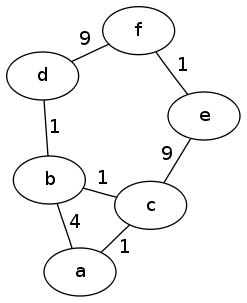
\includegraphics[width=4cm]{example.png}
\end{center}
\caption{Einfacher gewichteter Graph}
\vspace{-60pt}
\end{wrapfigure}

Knoten den Wert 0 zuweisen und einrahmen. \\ Verbundene Knoten beschriften: \emph{b = 4, c = 1}.

Tiefsten temporär beschrifteten Knoten einrahmen: \emph{c}. \\ Verbundene Knoten beschriften: \emph{b = 2, e = 10}.

Tiefsten temporär beschrifteten Knoten einrahmen: \emph{b}. \\ Verbundene Knoten beschriften: \emph{d = 3}.

Tiefsten temporär beschrifteten Knoten einrahmen: \emph{d}. \\ Verbundene Knoten beschriften: \emph{f = 12}.

Tiefsten temporär beschrifteten Knoten einrahmen: \emph{e}. \\ Verbundene Knoten beschriften: \emph{f = 11}.

Tiefsten temporär beschrifteten Knoten einrahmen: \emph{f}.

Der schnellste Weg lautet: \emph{f, e, c, a}.

\vspace{10pt}

Wie man leicht erkennen kann, wird der schnellste Weg gefunden, indem der Pfad welcher zum Einrahmen der jeweiligen Knoten geführt hat, rückwärts durchquert wird. Bei bedarf lässt sich dieser spiegeln, damit er beim Anfangsknoten beginnt und beim Zielknoten endet.

\section{Modell}

\subsection{Programmablauf}

\begin{wrapfigure}{lh!}{0.5\textwidth}
\begin{center}
	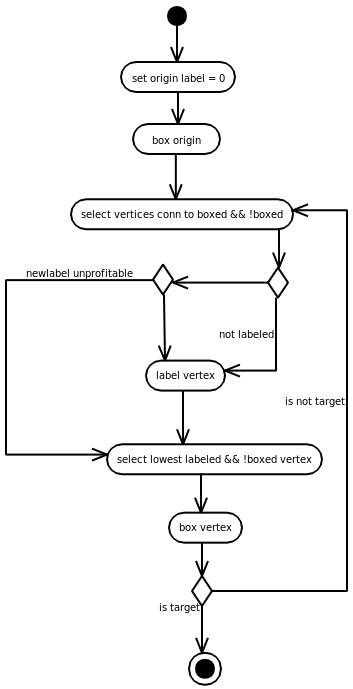
\includegraphics[width=7cm]{activity_diagram.png}
\end{center}
\caption{UML Aktivitätsdiagramm des Dijkstra}
\vspace{-60pt}
\end{wrapfigure}

Dieses Diagramm beschreibt den Ablauf des Dijkstra Algorithmus. Es entspricht der obrigen Definition.

\clearpage

\subsection{Datenmodell}

Es folgt ein Diagramm, welche die verwendeten Klassen, sowie deren Attribute und Beziehungen untereinander beschreibt. Diese Klassen definieren, welche Daten verwendet werden.

\begin{figure}[h]
\begin{center}
	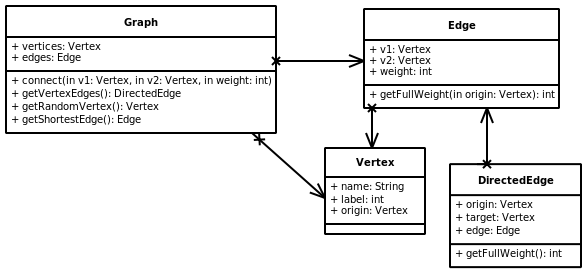
\includegraphics[width=0.7\textwidth]{model_diagram2.png}
\end{center}
\caption{UML Klassendiagramm des Modells}
\end{figure}

\newpage

\section{Dateiformat}

\subsection{Allgemein}

Damit es möglich ist Graphen in das Programm zu laden, braucht es ein Dateiformat. Der Einfachheit halber wird hier ein ASCII basiertes Format verwendet. Eine Zeile in der Datei kann hierbei entweder einen Knoten oder eine Kante beschreiben.

Die Zeilen werden mittels Linefeed (\emph{ASCII 10}) getrennt. Pro Zeile gibt es Tokens, die via Tab (\emph{ASCII 9}) getrennt werden. Dies gleicht einem CSV-Format mit Tab Delimiter.

\begin{figure}[hb]
\begin{tabbing}
	\hspace*{3em} \= \hspace{2.7em} \= \hspace{3.7em} \= \hspace{2.7em} \= \hspace{4.8em} \= \kill
	[typ] \> \fbox{tab} \> [token] \> \fbox{tab} \> [token\_n] \> \fbox{linefeed}
\end{tabbing}
\caption{Grundgerüst des Dateiformats}
\end{figure}

\subsection{Typen}

Ein \emph{v} als Typ steht für einen Knoten (\emph{Vertex}), ein \emph{e} für eine Kante (\emph{Edge}). Je nach Typ gibt es verschiedene Tokens.

\subsubsection{Vertex}

% ...

\newpage

\section{Pseudocode}

\newpage

\section{Programmdokumentation}

\newpage

\section{Reflexion}

\newpage

\section{Verwendete Mittel}

\subsection{Programme}

\begin{itemize}
\item \emph{\href{http://www.eclipse.org}{Eclipse}:} Entwicklungsumgebung für Java
\item \emph{\href{http://gaphor.sourceforge.net}{Gaphor}:} UML Diagramm Tool
\item \emph{\href{http://graphviz.org}{Graphviz}:} Graphenvisualisierung
\item \emph{\href{http://www.lcdf.org/gifsicle}{Gifsicle}:} Animierte gifs erstellen
\end{itemize}

\subsection{Quellen}

\subsubsection{WWW}

\begin{itemize}
\item \emph{\href{http://ocw.mit.edu/NR/rdonlyres/Sloan-School-of-Management/15-082JNetwork-OptimizationSpring2003/FC13EFA1-0FE2-4BFB-B019-8939606EDDCC/0/dijkstrasalgorithm.pdf}{Dijkstra’s Algorithm (PDF)}}
\item \emph{\href{http://www.educ.ethz.ch/lehrpersonen/informatik/unterrichtsmaterialien_inf/kommuniation_kryptographie/routing/la3.pdf}{Der Algorithmus von Dijkstra (PDF)}}
\item \emph{\href{http://en.wikipedia.org/wiki/ASCII}{ASCII - Wikipedia}}
\end{itemize}

\subsubsection{Literatur}
\begin{itemize}
\item \emph{Networks - Student text and unit guide, Cambridge 2000}
\item andere Unterlagen aus dem Unterricht
\end{itemize}

\end{document}
